\chapter{Existing Technology}

Variable pitch is not a new concept on quadcopters. The first quadcopter with variable pitch was built in the 1920s and was called the "de Bothezat helicopter". This helicopter is said to be the first successful helicopter of its time, but was discontinued due complexity, control difficulties, and high pilot workload. \cite{bothezat}
%\ref(https://en.wikipedia.org/wiki/De_Bothezat_helicopter)
Variable pitch has since the "de Bothezat helicopter" been used on all modern helicopters, as well as RC-helicopters. \\

Lately, variable pitch has gained popularity on small RC-quadcopters, but is still in the early stages of development. As of today, there are multiple commercially available pitch mechanisms and a few commercially available variable pitch quadcopters. As far as the authors know, there is no commercially available open source flight controller that supports variable pitch quadcopters.

\section{Variable Pitch Mechanisms}

A variable pitch mechanism, is a mechanism that transfers linear motion into rotational motion on the propeller blades and alters the propellers angle of attack. Changing pitch angle can increases or decreases the amount of thrust produced. The pitch angle may be changed without substantially changing the rotational speed of the motor, giving the possibility of near instant thrust changes. \\
\\
Pitch mechanisms can also create negative pitch angles, and thus produce negative thrust without changing the rotational direction of the propeller. This allows for the possibility to fly inverted and could also be used for rapid decelerations.\\
\\
Variable pitch mechanisms compatible with quadcopters are commercially available and comes in two main varieties, hollow shaft motor with co-axle or as helicopter tail pitch mechanisms. Helicopters also use variable pitch on their main rotor, but this mechanism is much more complex and has more degrees of freedom than that of a tail pitch mechanism. On the main rotor of a helicopter, the device is called a swash plate and can tilt the main blade in multiple directions giving the helicopter extended control bandwidth. For the purpose of building a variable pitch quadcopter, there is no need for a swash plate.

\section{Variable Pitch Propellers}
%technical - motor prop desciption

The airfoil of a propeller is a section of the cross sectional area of the propeller. This cross sectional geometry determines its aerodynamic properties.\\

%The chord line is a straight line connecting the leading and trailing edges of the airfoil.

Today, existing variable pitch quadcopters and helicopter tails use symmetric airfoils. This means that if a horizontal line (chord line) is drawn connecting the leading and trailing edges of the airfoil, the pieces above and below the line will be equal. 
Symmetric airfoils gives the possibility of producing equal amounts of thrust in either direction of pitch, allowing negative and positive thrust values and inverted flight.  
\\
If inverted flight is not of interest, non-symmetric airfoils may be used to increase upright flight efficiency.

%% Man kan 
% Hvis inverted flight ikke er interessant, kan man tenke seg å bruke en airfoil som er optimalisert for upward flight (med twist). 

\clearpage

\section{Helicopter Tail Rotor Mechanism}
The pitch of a helicopter tail blade is controlled by a servo. The servo applies rotational motion to a linkage rod which is connected to the tail rotor control arm. The rotational motion of the servo becomes linear motion in the linkage rod and the linkage rod pushes on the tail rotor control arm. The tail rotor control arm pivots about a point. When a force is applied to the tail rotor control arm, the arm raises or lowers the pitch slider on the rotating shaft. Thus, increasing or decreasing the angle of pitch. See Fig. \ref{fig:helitailrotor}.\\ 
\\
\begin{figure}[H]
\centering
    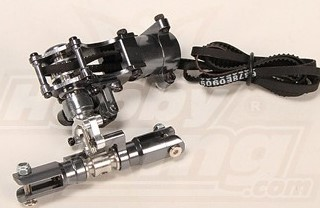
\includegraphics[width = 0.4\textwidth]{VAPIQ-PICTURES/hk500gt}
    \caption{HK500GT - Align T-Rex Tail Rotor Mechanisms}
    \label{fig:helitailrotor}    
\end{figure}

\section{Variable Pitch with Hollow Shafts}
The second type of mechanism available, is the hollow shaft mechanism, illustrated in Fig. \ref{fig:Axi220826}. In this type of mechanism, the motor has a hollow outer shaft. Within the hollow shaft, there is a inner slide shaft. The inner shaft slides freely within the hollow shaft. In this configuration, the servo is placed directly under the motor. The inner shaft is connected to a control link mechanism, which in turn is connected to the rotor holder. When a force is applied by the servo, the inner shaft slides up or down. This in turn rotates the rotor holder, changing the angle of pitch on the propellers. 

\begin{figure}[H]
\centering
    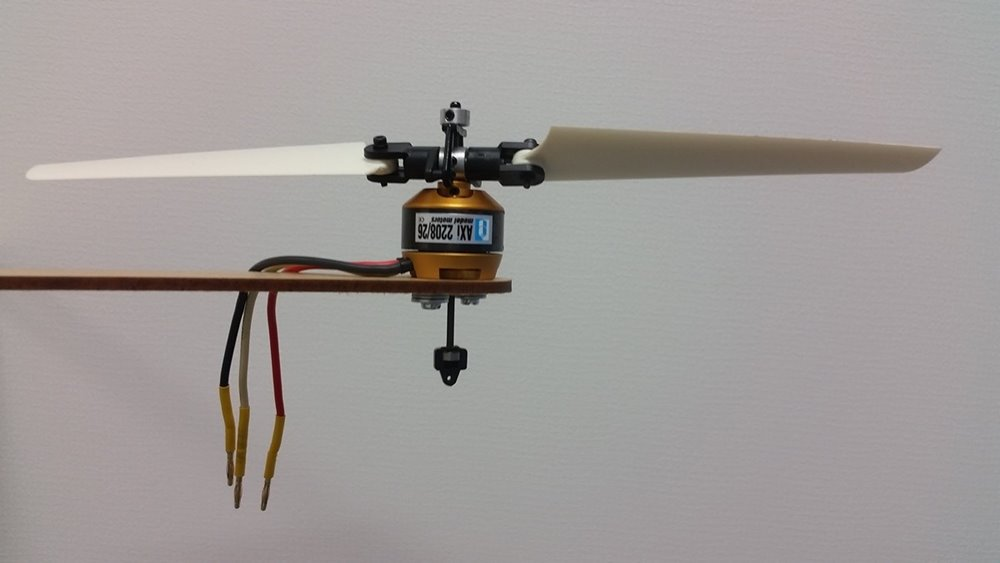
\includegraphics[width = 0.5\textwidth]{VAPIQ-PICTURES/Axi2208}
    \caption{Axi 2208/26 Hollow Shaft With Variable Pitch Mechanism}
    \label{fig:Axi220826}    
\end{figure}

\clearpage
\section {Variable Pitch Frame types}
There are two main configurations of quadcopters with variable pitch. The most common frame type is the \textbf{H-shape} frame with central motor and belt drive. 

\begin{figure}[H]
\centering
    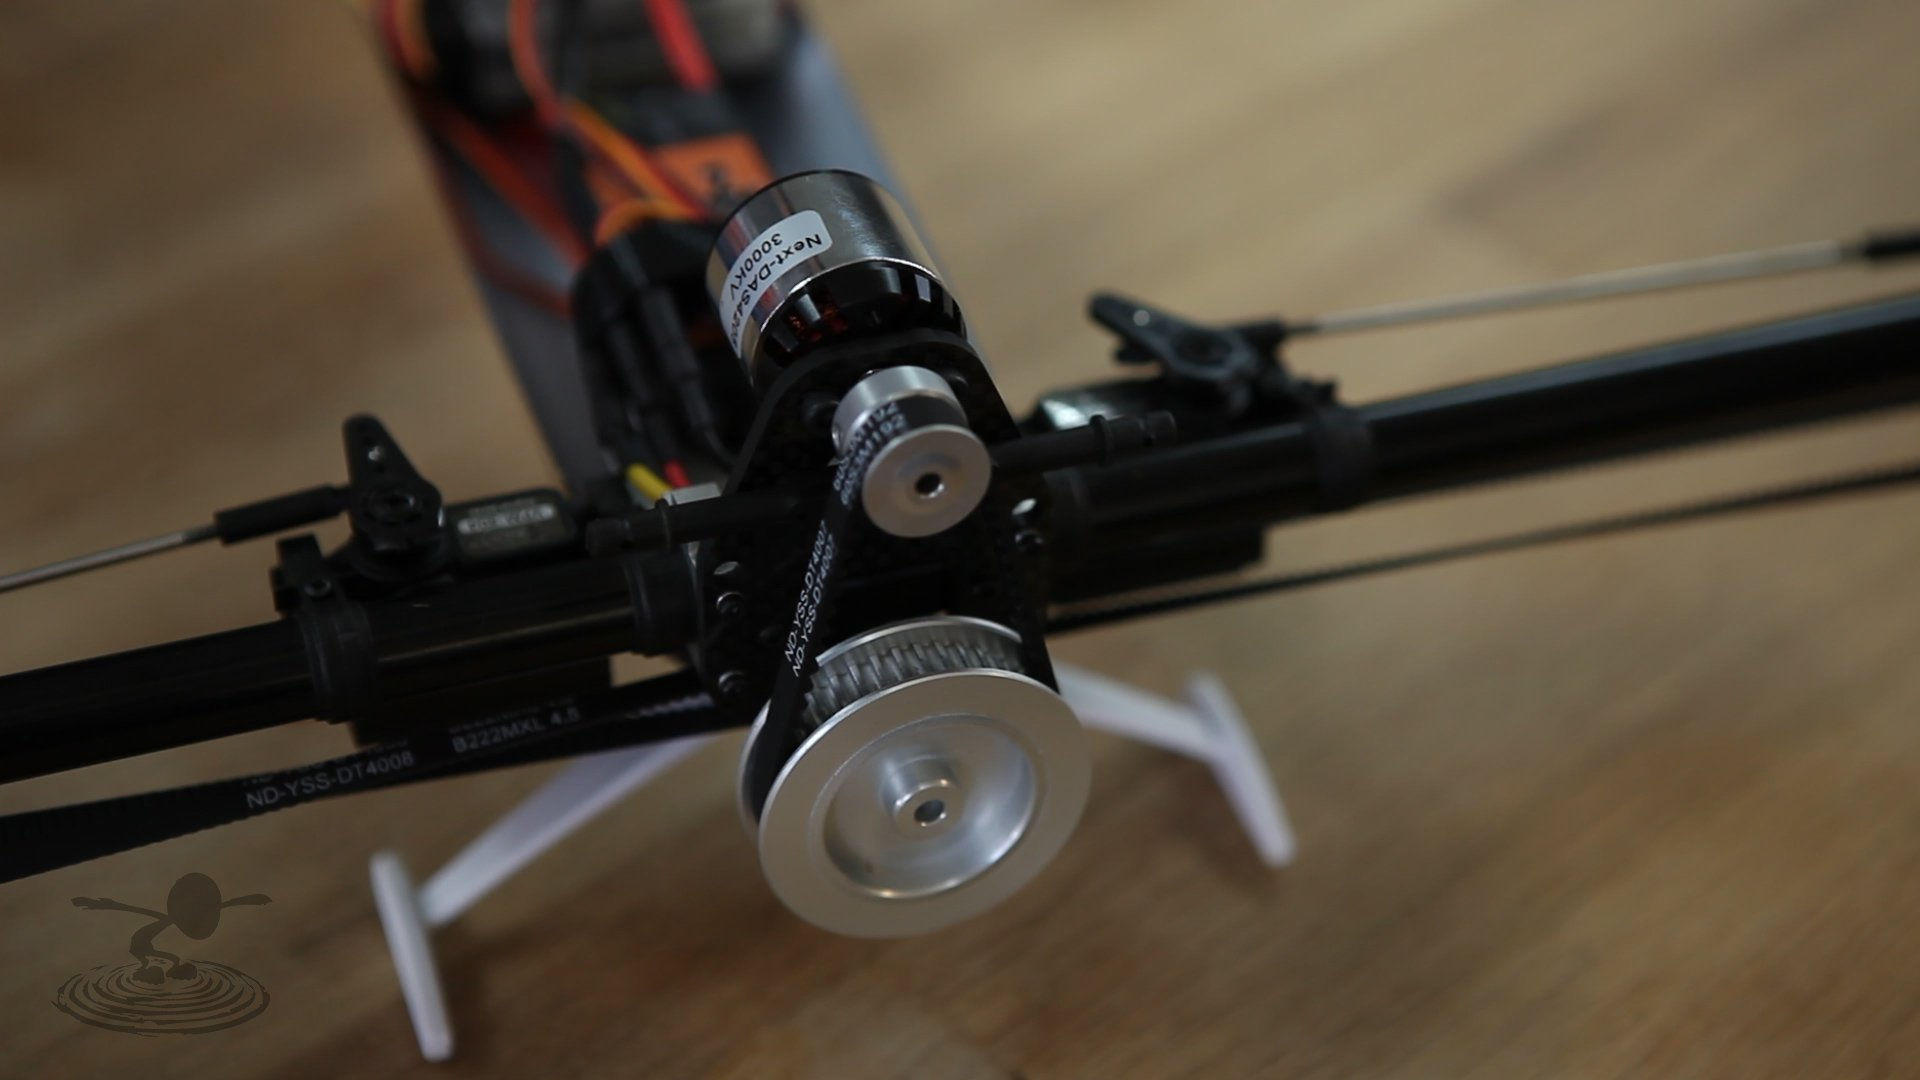
\includegraphics[width = 0.6\textwidth]{VAPIQ-PICTURES/hcop}
    \caption{Stingray 500 Motor and Belt System \cite{flitetest}}
    \label{fig:hcop}    
\end{figure}

The other type of frame is the more traditional \textbf{X-shaped} frame which can have central motor or four individual motors. The benefit of having individual motors is that you can control both RPM and pitch, giving the possibility of even more agile flight. On the downside, this may be a more power consuming configuration. \\

The most famous commercially available variable pitch quadcopter is the Curtis Youngblood - Stingray 500 shown in Fig. \ref{fig:stingray}. This is a quadcopter designed and built by Curtis Youngblood, and is said to be the first ever commercial collective pitch quadcopter \cite{curtis}.  

\begin{figure}[h]
\centering
    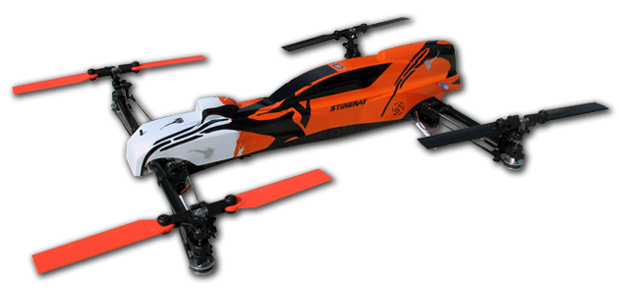
\includegraphics[scale = 1]{VAPIQ-PICTURES/stingray}
    \caption{Curtis Youngblood - Stingray 500}
    \label{fig:stingray}    
\end{figure}

The Stingray has a single central engine with 3000KV. The flight controller is specially developed and built from scratch just for this model, and is not open source.

 

